\documentclass[a4paper,10pt]{article}
\usepackage[a4paper, total={175mm, 245mm}]{geometry}

\usepackage[colorlinks,linkcolor=blue,bookmarks,bookmarksopen,pdfauthor=krom]{hyperref}

\usepackage{fontspec}
\setmainfont{epkyouka.ttf}

\graphicspath{{images/}}

\usepackage[normalem]{ulem}
\renewcommand{\ULthickness}{0.08em}

\usepackage[compact]{titlesec}
\titlespacing{\section}{0em}{*0}{1em}
\titlespacing{\subsection}{0em}{*0}{0em}
\titlespacing{\subsubsection}{0em}{*0}{0em}
\titleformat{\section}{\normalfont}{\thesection}{1em}{}
\titleformat{\subsection}{\normalfont}{\thesection}{1em}{}
\titleformat{\subsubsection}{\normalfont}{\thesection}{1em}{}

\usepackage[titles]{tocloft}
\renewcommand\cftsecdotsep{\cftdotsep}
\renewcommand\cfttoctitlefont{\normalfont}
\renewcommand\cftdot{…}
\renewcommand\cftdotsep{0}
\setlength\cftbeforesecskip{0em}
\setlength\cftaftertoctitleskip{1.5em}
\renewcommand{\cftsecafterpnum}{\hspace*{3em}}
\renewcommand{\cftsubsecafterpnum}{\hspace*{3em}}
\renewcommand{\cftsubsubsecafterpnum}{\hspace*{3em}}

\setlength\parindent{2.5em}
\setlength\parskip{0em}
\renewcommand{\baselinestretch}{1.6}

\usepackage{fancyhdr}
\pagestyle{fancy}
\fancyhf{}
\renewcommand\headrulewidth{0pt}

\usepackage{arydshln}

\usepackage{rotating}
\usepackage{tikz}
\usetikzlibrary{arrows,decorations.markings,positioning,calc}
\tikzset{>=latex} % Define Standard Arrow Tip
\tikzstyle{vecArrow} = [thick, decoration={markings,mark=at position 1 with {\arrow[ultra thin,scale=4.5]{open triangle 90}}},
   double distance=18pt, shorten >= 14.5pt,
   preaction = {decorate},
   postaction = {draw,line width=18pt, white,shorten >= 13.5pt}]
\tikzstyle{vecArrowBig} = [thick, decoration={markings,mark=at position 1 with {\arrow[ultra thin,scale=6]{open triangle 90}}},
   double distance=27pt, shorten >= 19.5pt,
   preaction = {decorate},
   postaction = {draw,line width=27pt, white,shorten >= 18.5pt}]
\tikzstyle{vecArrowSmall} = [thick, decoration={markings,mark=at position 1 with {\arrow[ultra thin,scale=3.5]{open triangle 90}}},
   double distance=12pt, shorten >= 11.4pt,
   preaction = {decorate},
   postaction = {draw,line width=12pt, white,shorten >= 10.4pt}]
\tikzstyle{innerWhite} = [semithick, white,line width=18pt, shorten >= 0pt]
\tikzstyle{innerWhiteBig} = [semithick, white,line width=27pt, shorten >= 0pt]
\tikzstyle{innerWhiteSmall} = [semithick, white,line width=12pt, shorten >= 0pt]

\usepackage{enumitem}

\usepackage{amsmath} % For \boxed{}

\frenchspacing

\begin{document}

\begin{picture}(0,0)
\put(-55,8){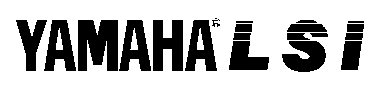
\includegraphics[width=19em]{YAMAHALSI}}
\put(-55,-208){
\includegraphics[width=50em]{V9958MSX-VIDEOTechnicalDataBook}}
\put(148,-685){
\includegraphics[width=11em]{YAMAHA}}
\end{picture}

\setcounter{page}{0}
\fancyfoot[R]{\vspace{-3.5em}
\setlength{\arrayrulewidth}{0.1em}
\setlength{\tabcolsep}{0.5em}
\renewcommand{\arraystretch}{0.3}
\begin{tabular}{|c|}
\hline
\\[-0.2em]
V9958TECHNICAL DATA BOOK\\
\hline
\\[-0.2em]
CATALOG No.:249958Y\\
\hline
\\[-0.2em]
1988.12\\
\hline
\end{tabular}
}

\newpage

\setcounter{page}{0}
\fancyfoot{}

\fontsize{11.2pt}{11.2pt}\selectfont

PREFACE\\
\par
This booklet describes those specifications which have been added, modified or\par
deleted on the basis of specifications of V9938. The ones not found here have\par
remained the same as V9938 but note that some, even the same, may be included\par
here due to the conveniance of editing. For specifications of V9938, refer to\par
\hskip -0.5em “V9938 MSX-VIDEO Technical Data Book".\\
\par
\hskip 22em December 1988 YAMAHA Corporation\par
\hskip 27em Semiconductor Division

\newpage

\setcounter{page}{0}

\renewcommand\contentsname{\hskip 6em TABLE OF CONTENTS}
\addtocontents{toc}{\hskip 37.75em Page\par}
\tableofcontents

\newpage

\setcounter{page}{1}
\fancyfoot[C]{\Large \thepage}

\phantomsection
\section*{\boxed{1}  GENERAL DESCRIPTION}
\addcontentsline{toc}{section}{\hskip 5.5em [1] \ GENERAL DESCRIPTION}

\noindent This LSI is a video display Processor(VDP) which is applicable to new\\
media. It uses an N-channel silicon gate MOS and has a linear RGB output.\\
It is software compatible with TMS9918A and V9938.\\

\phantomsection
\section*{\boxed{2}  FEATURES}
\addcontentsline{toc}{section}{\hskip 5.5em [2] \ FEATURES}

\renewcommand{\labelitemi}{・}
\begin{itemize}[leftmargin=1em, labelsep=0em, itemsep=-0.32em]
\item 5V power supply.
\item Outputs linear RGB.
\item Built-in color palette for display in up to 512 colors.
\item Capable of simultaneous display of 19,268 colors by using YJK system.\\
display.
\item Capable of displaying up to 512×424 Pixels and 16 colors.
\item Bit mapped graphics.
\item Capable of displaying maximum of 256 colors simultaneously.
\item 16K byte~128K byte useable for display memory.
\item 16K×1b,16K×4b,64K×1b and 64K×4b DRAMs are useable.
\item 256 addresses,4ms auto refresh function of DRAM.
\item Expansion video memory can be connected.
\item Eight sprites can be displayed for each horizontal line.
\item Colors for sprites can be specified for each horizontal line.
\item Area move, line, search and other commands.
\item Command function usable in every display mode.
\item Logical operation function.
\item Addresses can be specified by coordinates.
\item Capable of external synchronization.
\item Capable of superimposition.
\item Capable of digitization.
\item Multi MSX-VIDEO configurations are possible.
\item External color palettes can be added by utilizing color bus output.
\item Vertical and horizontal scroll function.
\item Wait function to CPU.
\end{itemize}

\newpage

\phantomsection
\section*{\boxed{3}  INTERNAL STRUCTURE BLOCK DIAGRAM}
\addcontentsline{toc}{section}{\hskip 5.5em [3] \ INTERNAL STRUCTURE BLOCK DIAGRAM}

\vspace{0.5em}
\hskip 3.2em \begin{sideways}

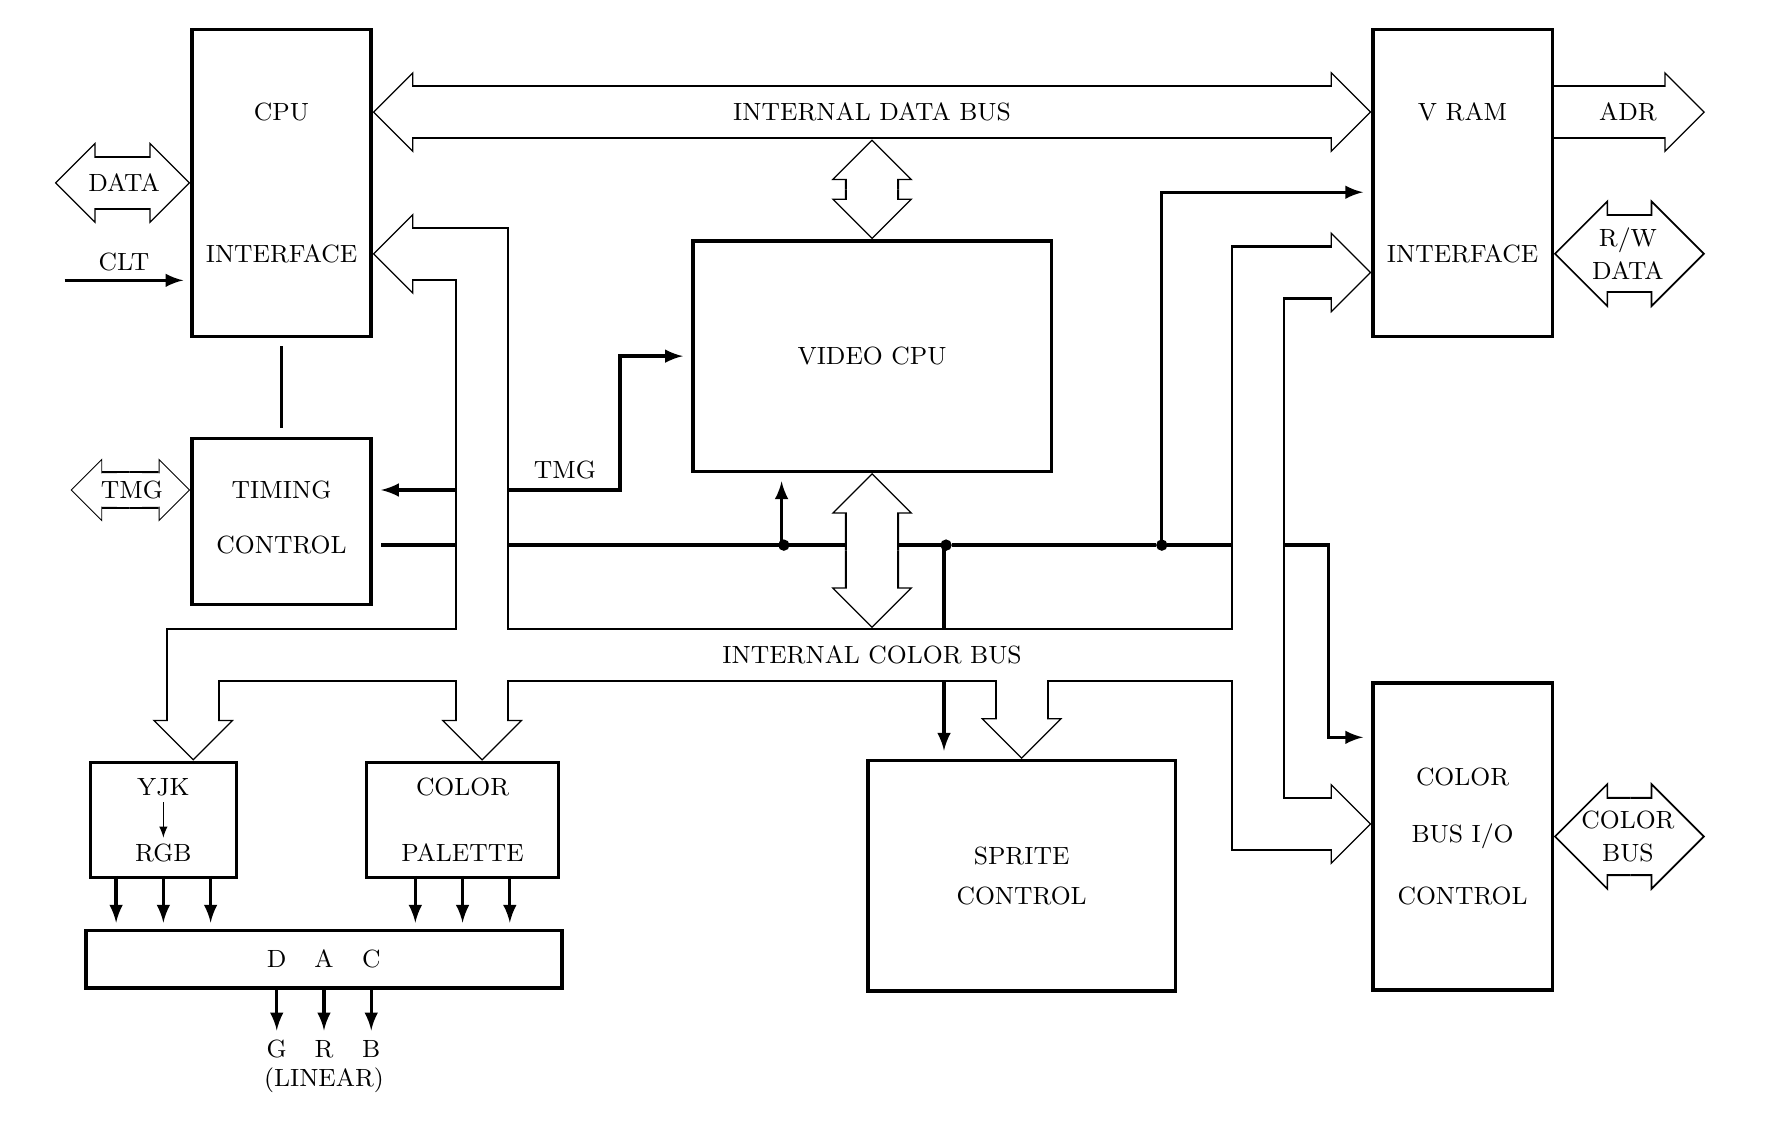
\begin{tikzpicture}[very thick]
\fontsize{9pt}{9pt}

\node[draw,rectangle,minimum width=7em,minimum height=12em,align=center] (VRAMINTERFACEBox) at (19.3,12.8) {};
\node[draw=none,fill=none,rectangle,minimum width=7em,minimum height=1em,align=center] (VRAM) at (19.3,13.7) {V RAM};
\node[draw=none,fill=none,rectangle,minimum width=7em,minimum height=1em,align=center] (VRAMINTERFACE) at (19.3,11.9) {INTERFACE};

\node[inner sep=0,minimum width=0,minimum height=0] (ADRInvisible) at (22.4,13.7) {};
\draw[vecArrow] (VRAM.east) to (ADRInvisible);
\node[inner sep=0,minimum width=0,minimum height=0] (ADR) at (21.4,13.7) {ADR};

\node[inner sep=0,minimum width=0,minimum height=0] (RWDATAInvisible) at (22.4,11.9) {};
\draw[vecArrowBig] ($(VRAMINTERFACE.east)!0.5!(RWDATAInvisible)$) to (RWDATAInvisible);
\draw[vecArrowBig] ($(VRAMINTERFACE.east)!0.5!(RWDATAInvisible)$) to (VRAMINTERFACE.east);
\draw[innerWhiteBig] ($(VRAMINTERFACE.east)!0.4!(RWDATAInvisible)$) to ($(VRAMINTERFACE.east)!0.6!(RWDATAInvisible)$);
\node[draw=none,fill=none,rectangle,minimum width=0,minimum height=0,align=center] (RWDATA) at (21.4,11.9) {R/W\\[-0.25em]DATA};

\node[draw,rectangle,minimum width=7em,minimum height=12em,align=center] (COLORBUSIOCONTROLBox) at (19.3,4.5) {};
\node[draw=none,fill=none,rectangle,minimum width=7em,minimum height=3em,align=center] (COLOR) at (19.3,5.25) {COLOR};
\node[draw=none,fill=none,rectangle,minimum width=7em,minimum height=1em,align=center] (BUSIO) at (19.3,4.5) {BUS I/O};
\node[draw=none,fill=none,rectangle,minimum width=7em,minimum height=1em,align=center] (COLORCONTROL) at (19.3,3.75) {CONTROL};

\node[inner sep=0,minimum width=0,minimum height=0] (COLORBUSInvisible) at (22.4,4.5) {};
\draw[vecArrowBig] ($(BUSIO.east)!0.5!(COLORBUSInvisible)$) to (COLORBUSInvisible);
\draw[vecArrowBig] ($(BUSIO.east)!0.5!(COLORBUSInvisible)$) to (BUSIO.east);
\draw[innerWhiteBig] ($(BUSIO.east)!0.4!(COLORBUSInvisible)$) to ($(BUSIO.east)!0.6!(COLORBUSInvisible)$);
\node[draw=none,fill=none,rectangle,minimum width=0,minimum height=0,align=center] (COLORBUS) at (21.4,4.5) {COLOR\\[-0.25em]BUS};

\node[draw,rectangle,minimum width=7em,minimum height=12em,align=center] (CPUINTERFACEBox) at (4.3,12.8) {};
\node[draw=none,fill=none,rectangle,minimum width=7em,minimum height=1em,align=center] (CPU) at (4.3,13.7) {CPU};
\node[draw=none,fill=none,rectangle,minimum width=7em,minimum height=1em,align=center] (CPUINTERFACE) at (4.3,11.9) {INTERFACE};

\draw[vecArrow] ($(CPU.east)!0.5!(VRAM.west)$) to (VRAM.west);
\draw[vecArrow] ($(CPU.east)!0.5!(VRAM.west)$) to (CPU.east);
\draw[innerWhite] ($(CPU.east)!0.4!(VRAM.west)$) to ($(CPU.east)!0.6!(VRAM.west)$);
\node[draw=none,fill=none,rectangle,minimum width=7em,minimum height=2em,align=center] (INTERNALDATABUS) at (11.8,13.7) {INTERNAL DATA BUS};

\node[inner sep=0,minimum width=0,minimum height=0] (DATAInvisible) at (1.4,12.8) {};
\draw[vecArrow] ($(CPUINTERFACEBox.west)!0.5!(DATAInvisible)$) to (DATAInvisible);
\draw[vecArrow] ($(CPUINTERFACEBox.west)!0.5!(DATAInvisible)$) to (CPUINTERFACEBox.west);
\draw[innerWhite] ($(CPUINTERFACEBox.west)!0.4!(DATAInvisible)$) to ($(CPUINTERFACEBox.west)!0.6!(DATAInvisible)$);
\node[inner sep=0,minimum width=0,minimum height=0] (DATA) at (2.3,12.8) {DATA};

\node[draw=none,fill=none,rectangle,minimum width=4.5em,minimum height=1em,align=center] (CLT) at (2.3,11.8) {CLT};
\draw[very thick,->] (CLT.south west) to (CLT.south east);

\node[draw,rectangle,minimum width=7em,minimum height=6.5em,align=center] (TIMINGCONTROLBox) at (4.3,8.5) {};
\node[draw=none,fill=none,rectangle,minimum width=7em,minimum height=1em,align=center] (TIMING) at (4.3,8.9) {TIMING};
\node[draw=none,fill=none,rectangle,minimum width=7em,minimum height=1em,align=center] (TIMINGCONTROL) at (4.3,8.2) {CONTROL};

\draw[shorten <= 3pt,shorten >= 3pt,very thick,-] (CPUINTERFACEBox.south) to (TIMINGCONTROLBox.north);

\node[inner sep=0,minimum width=0,minimum height=0] (TMGInvisible) at (1.6,8.9) {};
\draw[vecArrowSmall] ($(TIMING.west)!0.5!(TMGInvisible)$) to (TMGInvisible);
\draw[vecArrowSmall] ($(TIMING.west)!0.5!(TMGInvisible)$) to (TIMING.west);
\draw[innerWhiteSmall] ($(TIMING.west)!0.4!(TMGInvisible)$) to ($(TIMING.west)!0.6!(TMGInvisible)$);
\node[inner sep=0,minimum width=0,minimum height=0] (TMG) at (2.4,8.9) {TMG};

\node[draw,rectangle,minimum width=14em,minimum height=9em,align=center] (VIDEOCPU) at (11.8,10.6) {VIDEO CPU};

\draw[vecArrow] ($(INTERNALDATABUS.south)!0.5!(VIDEOCPU.north)$) to (VIDEOCPU.north);
\draw[vecArrow] ($(INTERNALDATABUS.south)!0.5!(VIDEOCPU.north)$) to (INTERNALDATABUS.south);
\draw[innerWhite] ($(INTERNALDATABUS.south)!0.4!(VIDEOCPU.north)$) to ($(INTERNALDATABUS.south)!0.6!(VIDEOCPU.north)$);

\node[inner sep=0,minimum width=0,minimum height=0] (TMGTextInvisible) at (8.6,8.9) {};
\draw[shorten >= 3pt,very thick,->] (TMGTextInvisible.east) to (TIMING.east);
\draw[shorten >= 3pt,very thick,->] (TMGTextInvisible.south) |- (VIDEOCPU.west);
\node[inner sep=0,minimum width=0,minimum height=0] (TMGText) at (7.9,9.15) {TMG};

\node[draw,rectangle,minimum width=12em,minimum height=9em,align=center] (SPRITECONTROL) at (13.7,4) {SPRITE\\CONTROL};

\draw[shorten <= 3pt,shorten >= 3pt,very thick,->] (TIMINGCONTROL.east) -| ($(VIDEOCPU.south west)!0.25!(VIDEOCPU.south east)$);
\node[draw,fill=black,inner sep=1pt,circle] (TIMINGCONTROLA) at (10.68,8.2) {};

\draw[shorten >= 3pt,very thick,->] (TIMINGCONTROLA) -| ($(SPRITECONTROL.north west)!0.25!(SPRITECONTROL.north east)$);
\node[draw,fill=black,inner sep=1pt,circle] (TIMINGCONTROLB) at (12.74,8.2) {};

\node[draw,fill=black,inner sep=1pt,circle] (TIMINGCONTROLC) at (15.48,8.2) {};
\draw[very thick,-] (TIMINGCONTROLB) to (TIMINGCONTROLC);
\draw[shorten >= 3pt,very thick,->] (TIMINGCONTROLC) |- ($(VRAMINTERFACEBox.north west)!0.53!(VRAMINTERFACEBox.south west)$);

\node[inner sep=0,minimum width=0,minimum height=0] (TIMINGCONTROLInvisible) at (17.6,8.2) {};
\draw[very thick,-] (TIMINGCONTROLC) to (TIMINGCONTROLInvisible.east);
\draw[shorten >= 3pt,very thick,->] (TIMINGCONTROLInvisible.north) |- (COLOR.north west);

\node[draw,rectangle,minimum width=7.5em,minimum height=4.5em,align=center] (COLORPALETTE) at (6.6,4.71) {COLOR\\[1em]PALETTE};
\node[draw,rectangle,minimum width=5.7em,minimum height=4.5em,align=center] (YJKRGB) at (2.8,4.71) {YJK\\[1em]RGB};
\node[draw,rectangle,minimum width=18.6em,minimum height=2.25em,align=center] (DACBox) at (4.84,2.94) {};
\draw[thin,->] ($(YJKRGB.north)!0.35!(YJKRGB.south)$) to ($(YJKRGB.north)!0.65!(YJKRGB.south)$);

\draw[shorten >= 3pt,very thick,->] (2.8,4) to (2.8,3.3);
\draw[shorten >= 3pt,very thick,->] (2.2,4) to (2.2,3.3);
\draw[shorten >= 3pt,very thick,->] (3.4,4) to (3.4,3.3);

\draw[shorten >= 3pt,very thick,->] (6.6,4) to (6.6,3.3);
\draw[shorten >= 3pt,very thick,->] (6,4) to (6,3.3);
\draw[shorten >= 3pt,very thick,->] (7.2,4) to (7.2,3.3);

\node[draw=none,fill=none,rectangle,minimum width=1.9em,minimum height=2.25em,align=center] (DACD) at (4.24,2.94) {D};
\node[draw=none,fill=none,rectangle,minimum width=1.9em,minimum height=2.25em,align=center] (DACA) at (4.84,2.94) {A};
\node[draw=none,fill=none,rectangle,minimum width=1.9em,minimum height=2.25em,align=center] (DACC) at (5.44,2.94) {C};

\node[draw=none,fill=none,rectangle,minimum width=1.9em,minimum height=1em,align=center] (GRBG) at (4.24,1.8) {G};
\node[draw=none,fill=none,rectangle,minimum width=1.9em,minimum height=1em,align=center] (GRBR) at (4.84,1.8) {R};
\node[draw=none,fill=none,rectangle,minimum width=1.9em,minimum height=1em,align=center] (GRBB) at (5.44,1.8) {B};

\draw[very thick,->] (DACD) to (GRBG);
\draw[very thick,->] (DACA) to (GRBR);
\draw[very thick,->] (DACC) to (GRBB);
\node[inner sep=0,minimum width=0,minimum height=0] (LINEAR) at (4.84,1.4) {(LINEAR)};

\node[inner sep=0,minimum width=0,minimum height=0] (INTERNALCOLORBUSInvisible) at (16.7,6.8) {};
\draw[vecArrow] (INTERNALCOLORBUSInvisible) -| ($(YJKRGB.north west)!0.7!(YJKRGB.north east)$);
\draw[vecArrow] (INTERNALCOLORBUSInvisible) -| ($(COLORPALETTE.north west)!0.6!(COLORPALETTE.north east)$);
\draw[vecArrow] (INTERNALCOLORBUSInvisible) -| (SPRITECONTROL.north);
\draw[vecArrow] (INTERNALCOLORBUSInvisible.north) |- ($(COLORBUSIOCONTROLBox.north west)!0.46!(COLORBUSIOCONTROLBox.south west)$);
\draw[vecArrow] (INTERNALCOLORBUSInvisible.south) |- (VRAMINTERFACE.south west);

\node[inner sep=0,minimum width=0,minimum height=0] (COLORPALETTEInvisible) at (6.85,6.8) {};
\draw[vecArrow] (COLORPALETTEInvisible) |- (CPUINTERFACE.east);
\draw[innerWhite] ($(COLORPALETTEInvisible.west)!1.032!(INTERNALCOLORBUSInvisible)$) to ($(INTERNALCOLORBUSInvisible)!1.2!(COLORPALETTEInvisible.west)$);

\node[draw=none,fill=none,rectangle,minimum width=7em,minimum height=2em,align=center] (INTERNALCOLORBUS) at (11.8,6.8) {INTERNAL COLOR BUS};
\draw[vecArrow] ($(INTERNALCOLORBUS.north)!0.5!(VIDEOCPU.south)$) to (VIDEOCPU.south);
\draw[vecArrow] ($(INTERNALCOLORBUS.north)!0.5!(VIDEOCPU.south)$) to (INTERNALCOLORBUS.north);
\draw[innerWhite] ($(INTERNALCOLORBUS.north)!0.4!(VIDEOCPU.south)$) to ($(INTERNALCOLORBUS.north)!0.6!(VIDEOCPU.south)$);
\end{tikzpicture}

\end{sideways}

\newpage

\phantomsection
\section*{\boxed{4}  PIN LAYOUT AND FUNCTIONS}
\addcontentsline{toc}{section}{\hskip 5.5em [4] \ PIN LAYOUT AND FUNCTIONS}

\vspace{1.5em}

\fontsize{10pt}{10pt}\selectfont
\setlength{\arrayrulewidth}{0.1em}
\setlength{\tabcolsep}{0.5em}
\renewcommand{\arraystretch}{1.4}
\noindent \begin{tabular}{|c|c|c|l|}
\hline
\ Pin Name \ & Pin No. & \ \ I/O \ \ & \ \ \ \ \ \ \ \ \ \ \ \ \ \ \ \ \ \ \ \ \ \ \ \ \ \ \ \ \ \ \ Function \ \ \ \ \ \ \ \ \ \ \ \ \ \ \ \ \ \ \ \ \ \ \ \ \ \ \ \ \ \ \ \\
\hline \\[-2.8em]
CD0 LSB & 40 & I/O & CPU data bus\\[-1.04em]
CD1 & 39 & I/O & \ \ \ \ \ "\\[-1.04em]
CD2 & 38 & I/O & \ \ \ \ \ "\\[-1.04em]
CD3 & 37 & I/O & \ \ \ \ \ "\\[-1.04em]
CD4 & 36 & I/O & \ \ \ \ \ "\\[-1.04em]
CD5 & 35 & I/O & \ \ \ \ \ "\\[-1.04em]
CD6 & 34 & I/O & \ \ \ \ \ "\\[-1.04em]
CD7 MSB & 32 & I/O & \ \ \ \ \ "\\[-1.04em]
MODE 0 & 29 & I & CPU interface mode select\\[-1.04em]
MODE 1 & 28 & I & \ \ \ \ \ "\\[-1.04em]
$\overline{\mbox{CSR}}$ & 31 & I & CPU-MSX-VIDEO read strobe\\[-1.04em]
$\overline{\mbox{CSW}}$ & 30 & I & CPU-MSX-VIDEO write strobe\\[-1.04em]
RD0 LSB & 41 & I/O & VRAM data bus\\[-1.04em]
RD1 & 42 & I/O & \ \ \ \ \ "\\[-1.04em]
RD2 & 43 & I/O & \ \ \ \ \ "\\[-1.04em]
RD3 & 44 & I/O & \ \ \ \ \ "\\[-1.04em]
RD4 & 45 & I/O & \ \ \ \ \ "\\[-1.04em]
RD5 & 46 & I/O & \ \ \ \ \ "\\[-1.04em]
RD6 & 47 & I/O & \ \ \ \ \ "\\[-1.04em]
RD7 MSB & 48 & I/O & \ \ \ \ \ "\\[-1.04em]
AD0 LSB & 49 & O & VRAM address bus\\[-1.04em]
AD1 & 50 & O & \ \ \ \ \ "\\[-1.04em]
AD2 & 51 & O & \ \ \ \ \ "\\[-1.04em]
AD3 & 52 & O & \ \ \ \ \ "\\[-1.04em]
AD4 & 53 & O & \ \ \ \ \ "\\[-1.04em]
AD5 & 54 & O & \ \ \ \ \ "\\[-1.04em]
AD6 & 55 & O & \ \ \ \ \ "\\[-1.04em]
AD7 MSB & 56 & O & \ \ \ \ \ "\\[-1.04em]
$\overline{\mbox{RAS}}$ & 62 & O & VRAM row address strobe\\[-1.04em]
$\overline{\mbox{CAS 0}}$ & 61 & O & VRAM column address strobe 0 (first half of VRAM)\\[-1.04em]
$\overline{\mbox{CAS 1}}$ & 60 & O & VRAM column address strobe 1 (last half of VRAM)\\[-1.04em]
$\overline{\mbox{CAS X}}$ & 59 & O & VRAM column address strobe X (for expansion VRAM)\\[-1.04em]
R/$\overline{\mbox{W}}$ & 57 & O & VRAM write strobe\\[-1.04em]
G & 22 & O & Linear RGB signal output\\[-1.04em]
R & 23 & O & \ \ \ \ \ "\\[-1.04em]
B & 24 & O & \ \ \ \ \ "\\[-1.04em]
$\overline{\mbox{YS}}$ & 10 & O & Signal for switching between MSX-VIDEO RGB output and external video\\[-1.04em]
& & & signals. (For superimpose)\\[-1.04em]
& & & \ $\overline{\mbox{YS}}$ = High: MSX-VIDEO output is transparent\\[-1.04em]
& & & \ $\overline{\mbox{YS}}$ = Low : MSX-VIDEO output is not transparent\\[-1.04em]
BLEO & 7 & O & Indicates No. 1 field/No. 2 field blanking with 3-value output.\\[-1.04em]
& & & \ \ \ \ \ \ Open drain output\\[-1.04em]
& & & \ \ \ \ \ \ High \ : No. 2 field and active.\\[-1.04em]
& & & \ \ \ \ \ \ Middle: No. 1 field and active.\\[-1.04em]
& & & \ \ \ \ \ \ Low \ \ : Linear erase interval.\\
\hline
\end{tabular}

\newpage

\fontsize{10pt}{10pt}\selectfont
\setlength{\arrayrulewidth}{0.1em}
\setlength{\tabcolsep}{0.5em}
\renewcommand{\arraystretch}{1.4}
\noindent \begin{tabular}{|c|c|c|l|}
\hline
\ Pin Name \ & Pin No. & \ \ I/O \ \ & \ \ \ \ \ \ \ \ \ \ \ \ \ \ \ \ \ \ \ \ \ \ \ \ \ \ \ \ \ \ \ Function \ \ \ \ \ \ \ \ \ \ \ \ \ \ \ \ \ \ \ \ \ \ \ \ \ \ \ \ \ \ \ \\
\hline \\[-2.8em]
$\overline{\mbox{HSYNC}}$ & 5 & O & High: Timing other than HSYNC or color burst timing.\\[-1.04em]
& & & Low : HSYNC or timing other than color burst.\\[-1.04em]
$\overline{\mbox{CSYNC}}$ & 6 & O & Composite SYNC output.\\[-1.04em]
CBDR & 11 & O & Indicates color bus direction.\\[-1.04em]
& & & \ \ \ \ High: Color bus is input\\[-1.04em]
& & & \ \ \ \ Low : Color bus is output\\[-1.04em]
C0 LSB & 19 & I/O & Color bus.\\[-1.04em]
C1 & 18 & I/O & Normally color code is output. Used as input port when digitizing.\\[-1.04em]
C2 & 17 & I/O & \ \ \ \ \ \ \ \ \ \ \ \ \ \ \ \ \ \ "\\[-1.04em]
C3 & 16 & I/O & \ \ \ \ \ \ \ \ \ \ \ \ \ \ \ \ \ \ "\\[-1.04em]
C4 & 15 & I/O & \ \ \ \ \ \ \ \ \ \ \ \ \ \ \ \ \ \ "\\[-1.04em]
C5 & 14 & I/O & \ \ \ \ \ \ \ \ \ \ \ \ \ \ \ \ \ \ "\\[-1.04em]
C6 & 13 & I/O & \ \ \ \ \ \ \ \ \ \ \ \ \ \ \ \ \ \ "\\[-1.04em]
C7 MSB & 12 & I/O & \ \ \ \ \ \ \ \ \ \ \ \ \ \ \ \ \ \ "\\[-1.04em]
$\overline{\mbox{DHCLK}}$ & 2 & O & Dot clock output at high resolution.\\[-1.04em]
& & & Approx. 10.74MHz open drain output.\\[-1.04em]
$\overline{\mbox{DLCLK}}$ & 3 & O & Dot clock output at low resolution.\\[-1.04em]
& & & Approx. 5.37MHz open drain output.\\[-1.04em]
& & & As input is also possible by using the mode register, it is used for\\[-1.04em]
& & & multi MSX-VIDEO.\\[-1.04em]
XTAL 1 & 63 & I & Used for XTAL connection. Also used for input when using an externally\\[-1.04em]
& & & generated clock.\\[-1.04em]
XTAL 2 & 64 & I &\\[-1.04em]
CPUCLK/ & 8 & O & 1/6 of XTAL frequency is output.\\[-1.04em]
$\overline{\mbox{VDS}}$ & & & \ VRAM data select\\[-1.04em]
& & & \ $\overline{\mbox{VDS}}$ = Low : VRAM access for display data.\\[-1.04em]
& & & \ $\overline{\mbox{VDS}}$ = High: VRAM access for other than the above.\\[-1.04em]
$\overline{\mbox{INT}}$ & 25 & O & CPU interrupt output, open drain output\\[-1.04em]
& & & Low: Generates interrupt.\\[-1.04em]
$\overline{\mbox{RESET}}$ & 9 & I & Each circuit in MSX-VIDEO is initial reset.\\[-1.04em]
$\overline{\mbox{VRESET}}$ & 4 & I & VSYNC input.\\[-1.04em]
$\overline{\mbox{HRESET}}$ & 27 & I & HSYNC input.\\[-1.04em]
$\overline{\mbox{WAIT}}$ & 26 & O & Wait signal to CPU is output.\\[-1.04em]
V\scriptsize{DD} & 58 & I & 5V power supply.\\[-1.04em]
GND & 1 & I & Ground 0V.\\[-1.04em]
GND$\bullet$DAC & 20 & I & Ground 0V.\\[-1.04em]
V\scriptsize{DD}\normalsize{$\bullet$DAC} & 21 & I & 5V power supply.\\[-1.04em]
V\scriptsize{BB} & 33 & I & Baseboard voltage.\\
\hline
\end{tabular}

\newpage

\fontsize{11.2pt}{11.2pt}\selectfont

\phantomsection
\section*{\boxed{5}  REGISTER DESCRIPTION}
\addcontentsline{toc}{section}{\hskip 5.5em [5] \ REGISTER DESCRIPTION}

\phantomsection
\subsection*{5-1 \, Added Registers}
\addcontentsline{toc}{subsection}{\hskip 5.7em 5-1 Added Registers}

Shown below are the registers newly added to the existing V9938 registers.\par

\vspace{0.2em}
\setlength{\arrayrulewidth}{0.1em}
\setlength{\tabcolsep}{0.5em}
\renewcommand{\arraystretch}{1}
\hskip -0.5em \begin{tabular}{c|c|c|c|c|c|c|c|c|}
\multicolumn{1}{c}{} & \multicolumn{1}{c}{\ \ b7 \ \ } & \multicolumn{1}{c}{\ \ b6 \ \ } & \multicolumn{1}{c}{\ \ b5 \ \ } & \multicolumn{1}{c}{\ \ b4 \ \ } & \multicolumn{1}{c}{\ \ b3 \ \ } & \multicolumn{1}{c}{\ \ b2 \ \ } & \multicolumn{1}{c}{\ \ b1 \ \ } & \multicolumn{1}{c}{\ \ b0 \ \ }\\
\cline{2-9}
♯25 & & CMD \ & VDS \ & YAE \ & YJK \ & WTE \ & MSK \ & SP2 \ \\
\cline{2-9}
\multicolumn{9}{c}{}\\[-0.8em]
\cline{2-9}
♯26 & & & HO8 \ & HO7 \ & HO6 \ & HO5 \ & HO4 \ & HO3 \ \\
\cline{2-9}
\multicolumn{9}{c}{}\\[-0.8em]
\cline{2-9}
♯27 & & & & & & HO2 \ & HO1 \ & HO0 \ \\
\cline{2-9}
\end{tabular}\\[0.5em]

The above three registers are cleared to“0" by the RESET signal and if\par
used in that state, will function compatibly with V9938.\\[-3.5em]

\[
\left.
\hskip 3em \begin{tabular}{l}
♯25 \ b7\\
♯26 \ b6, b7\\
♯27 \ b3~b7 \ \\
\end{tabular}
\right \} {\mbox{Make sure to set“0" for these empty bit positions.}}
\] 

\phantomsection
\subsubsection*{\ \ 5-1-1 \, Horizontal Scroll Function.}
\addcontentsline{toc}{subsubsection}{\hskip 4.15em 5-1-1 Horizontal Scroll Function}

\setlength{\arrayrulewidth}{0.1em}
\setlength{\tabcolsep}{0.5em}
\renewcommand{\arraystretch}{1}
\hskip -0.5em \begin{tabular}{c|c|c|c|c|c|c|c|c|l}
\multicolumn{1}{c}{} & \multicolumn{1}{c}{\ \ b7 \ \ } & \multicolumn{1}{c}{\ \ b6 \ \ } & \multicolumn{1}{c}{\ \ b5 \ \ } & \multicolumn{1}{c}{\ \ b4 \ \ } & \multicolumn{1}{c}{\ \ b3 \ \ } & \multicolumn{1}{c}{\ \ b2 \ \ } & \multicolumn{1}{c}{\ \ b1 \ \ } & \multicolumn{1}{c}{\ \ b0 \ \ } & \multicolumn{1}{c}{}\\
\cline{2-9}
♯25 & & & & & & & MSK \ & SP2 \ &\\
\cline{2-9}
\multicolumn{10}{c}{}\\[-0.8em]
\cline{2-9}
♯26 & & & HO8 \ & HO7 \ & HO6 \ & HO5 \ & HO4 \ & HO3 \ & by character\\
\cline{2-9}
\multicolumn{10}{c}{}\\[-2.5em]
\multicolumn{9}{c}{} & \multicolumn{1}{l}{units}\\[0.1em]
\cline{2-9}
♯27 & & & & & & HO2 \ & HO1 \ & HO0 \ & by dot units\\
\cline{2-9}
\end{tabular}\\[0.5em]

\hskip -0.5em HO8-HO0 \ \ Used to set the scroll volume of still pictures in the horizontal\par
\ \ \ \ \ \ \ \ \ \ direction one dot at a time.\par
\ \ \ \ \ \ \ \ \ \ \ (In G5 and G6 modes, scrolling is in 2-dot units.)\par
\ \ \ \ SP2 \ 0:Sets the horizontal screen size to 1 page. (Initial value)\par
\ \ \ \ \ \ \ \ \ \ \ \ \ Scrolling is done within one page and the non-displayed left\par
\ \ \ \ \ \ \ \ \ \ \ \ \ side of the page is displayed on the right hand side of the\par
\ \ \ \ \ \ \ \ \ \ \ \ \ screen.\par
\ \ \ \ \ \ \ \ \ 1:Sets the horizontal screen size to two pages.\par
\ \ \ \ \ \ \ \ \ \ \ \ \ Scrolling is done within 2 pages and if the first page is\par
\ \ \ \ \ \ \ \ \ \ \ \ \ displayed first, then the second page will appear at the\par
\ \ \ \ \ \ \ \ \ \ \ \ \ scroll operation.\par
\ \ \ \ MSK \ 0:The left 8 dots are not masked. \ (Initial value)\par
\ \ \ \ \ \ \ \ \ 1:The left 8 dots are masked and the border color is output.\par
\ \ \ \ \ \ \ \ \ \ \ \ \ There is no need to mask if the value in \#27 is“0".\par
\ \ \ \ \ \ \ \ \ \ \ \ \ (In G5 and G6 modes, the number of masked dots is 16.)\par

\newpage

\setlength{\arrayrulewidth}{0.1em}
\setlength{\tabcolsep}{0.5em}
\renewcommand{\arraystretch}{1}
\hskip 5.5em \begin{tabular}{|l|}
\hline
\ \ During scrolling, once the dots disappear to the left of the\\
\ \ screen or once the dots 1 to 7 appear on the screen, their data \ \\
\ \ are not controlled by V9958 and there is no guarantee on what\\
\ \ will be displayed.\\
\ \ To ensure proper display on the screen, therefore, masking is\\
\ \ necessary.\\
\hline
\end{tabular}\\[1em]

◎ Screen display for HO8-HO3\par
\ \ \ \ \ \ The screen is shifted \uline{to the left as }specified in 8-dot units\par
\ \ \ \ \ \ (in G5 and G6 modes, the screen is shifted in 16-dot units).\\
\par
・When SP2=0\par

\vspace{0.5em}
\setlength{\arrayrulewidth}{0.1em}
\setlength{\tabcolsep}{0.5em}
\renewcommand{\arraystretch}{1}
\hskip 1em \begin{tabular}{rr|c|c|cc|c|c|l}
\multicolumn{9}{l}{\ \ \ \ \ \ \ \ \ \ \ \ \ \ \ \ \ \ \ \ \ \ \ \ \ \ \ \ \ \ Display screen}\\
\cline{3-8}
\multicolumn{2}{r|}{HO7-3 \ \ \ } & \multicolumn{6}{|l|}{8 dots} &\\[-0.7em]
\multicolumn{9}{c}{}\\[-0.8em]
\cline{3-8}
\multicolumn{2}{r|}{0 \ \ \ \ \ } & \,0\, & \,1\, & \ \ \ \ \ \ \ \ \ \ \ \ \ \ \, & \ \ \ \ \ \ \ \ \ \ \ \ \ \ \, & 30 & 31 & 1 line\\
\cline{3-8}
\multicolumn{9}{c}{}\\[-0.8em]
\cline{3-8}
\multicolumn{2}{r|}{1 \ \ \ \ \ } & \,1\, & \,2\, & \ \ \ \ \ \ \ \ \ \ \ \ \ \ \, & \ \ \ \ \ \ \ \ \ \ \ \ \ \ \, & 31 & \,0\, &\\
\cline{3-8}
\multicolumn{1}{r;{1pt/3pt}}{\ \ \, } & \multicolumn{3}{c}{} & \multicolumn{1}{c;{1pt/3pt}}{} & \multicolumn{4}{c}{}\\
\multicolumn{1}{r;{1pt/3pt}}{} & \multicolumn{3}{c}{} & \multicolumn{1}{c;{1pt/3pt}}{} & \multicolumn{4}{c}{}\\
\multicolumn{1}{r;{1pt/3pt}}{} & \multicolumn{3}{c}{} & \multicolumn{1}{c;{1pt/3pt}}{} & \multicolumn{4}{c}{}\\
\cline{3-8}
\multicolumn{2}{r|}{31 \ \ \ \ \ } & 31 & \,0\, & \ \ \ \ \ \ \ \ \ \ \ \ \ \ \, & \ \ \ \ \ \ \ \ \ \ \ \ \ \ \, & 29 & 30 &\\
\cline{3-8}
\end{tabular}\\[0.5em]

\ \ \ \ \ \ \ \ \ \ \ \ Note) HO8 is ignored\par

\vspace{1em}

・When SP2=1\par

\vspace{-0.5em}
\setlength{\arrayrulewidth}{0.1em}
\setlength{\tabcolsep}{0.5em}
\renewcommand{\arraystretch}{1}
\hskip 1em \begin{tabular}{rr|c|c|c|c|c|c|c|c|l}
\multicolumn{11}{l}{\ \ \ \ \ \ \ \ \ \ \ \ \ \ \ \ \ \ Display screen}\\
\cline{3-6}
\multicolumn{2}{r|}{HO8-3 \ \ \ } & \multicolumn{4}{|l|}{8 dots} & \multicolumn{5}{c}{}\\[-0.7em]
\multicolumn{11}{c}{}\\[-0.8em]
\cline{3-10}
\multicolumn{2}{r|}{0 \ \ \ \ \ } & \,0\, & \,1\, & \ \ \ \ \ \ \ \ \ \ \, & 31 & 32 & \ \ \ \ \ \ \ \ \ \ \, & 62 & 63 & 1 line\\
\cline{3-10}
\multicolumn{11}{c}{}\\[-0.8em]
\cline{3-10}
\multicolumn{2}{r|}{1 \ \ \ \ \ } & \,1\, & \,2\, & \ \ \ \ \ \ \ \ \ \ \, & 32 & 33 & \ \ \ \ \ \ \ \ \ \ \, & 63 & \,0\, &\\
\cline{3-10}
\multicolumn{1}{r;{1pt/3pt}}{\ \ \, } & \multicolumn{4}{c}{} & \multicolumn{1}{c;{1pt/3pt}}{} & \multicolumn{5}{c}{}\\
\multicolumn{1}{r;{1pt/3pt}}{} & \multicolumn{4}{c}{} & \multicolumn{1}{c;{1pt/3pt}}{} & \multicolumn{5}{c}{}\\
\multicolumn{1}{r;{1pt/3pt}}{} & \multicolumn{4}{c}{} & \multicolumn{1}{c;{1pt/3pt}}{} & \multicolumn{5}{c}{}\\
\cline{3-10}
\multicolumn{2}{r|}{31 \ \ \ \ \ } & 31 & 32 & \ \ \ \ \ \ \ \ \ \ \, & 62 & 63 & \ \ \ \ \ \ \ \ \ \ \, & 29 & 30 &\\
\cline{3-10}
\multicolumn{11}{c}{}\\[-0.8em]
\cline{3-10}
\multicolumn{2}{r|}{32 \ \ \ \ \ } & 32 & 33 & \ \ \ \ \ \ \ \ \ \ \, & 63 & \,0\, & \ \ \ \ \ \ \ \ \ \ \, & 30 & 31 &\\
\cline{3-10}
\multicolumn{1}{r;{1pt/3pt}}{\ \ \, } & \multicolumn{4}{c}{} & \multicolumn{1}{c;{1pt/3pt}}{} & \multicolumn{5}{c}{}\\
\multicolumn{1}{r;{1pt/3pt}}{} & \multicolumn{4}{c}{} & \multicolumn{1}{c;{1pt/3pt}}{} & \multicolumn{5}{c}{}\\
\multicolumn{1}{r;{1pt/3pt}}{} & \multicolumn{4}{c}{} & \multicolumn{1}{c;{1pt/3pt}}{} & \multicolumn{5}{c}{}\\
\cline{3-10}
\multicolumn{2}{r|}{63 \ \ \ \ \ } & 63 & \,0\, & \ \ \ \ \ \ \ \ \ \ \, & 30 & 31 & \ \ \ \ \ \ \ \ \ \ \, & 61 & 62 &\\
\cline{3-10}
\end{tabular}

\newpage

\end{document}